\documentclass[italian,12pt,a4paper]{article}
\usepackage[utf8]{inputenc}
\usepackage[T1]{fontenc}
\usepackage{babel}
\usepackage{graphicx}
\usepackage{hyperref}
\usepackage{tikz}
\usepackage{pgf-pie}
\definecolor{myblue}{rgb}{0.152,0.690,0.894} %39,176,228
\definecolor{mygrey}{rgb}{0.062, 0.419,0.639}
\title{Università degli studi di Bari facoltà di scienze MM.FF.NN}
\date{} % clear date
\hypersetup{
	colorlinks=true,
	linkcolor=black,
	filecolor=magenta,      
	urlcolor=cyan,
	pdfpagemode=FullScreen,
}
\graphicspath{ {./images/} }
\usepackage{tocloft}


\cftsetindents{section}{0em}{2em}
\cftsetindents{subsection}{0em}{2em}

\renewcommand\cfttoctitlefont{\hfill\Large\bfseries}
\renewcommand\cftaftertoctitle{\hfill\mbox{}}

\setcounter{tocdepth}{2}
\begin{document}
	\maketitle
	\thispagestyle{empty}
	\begin{center}
		\huge	\textbf{Progetto Data Mining} \\
		\Large \textbf{NASA - Nearest Earth Objects hazard detection}
	\end{center}
	
	
	
	\begin{center}
		by \\
		\Large \textbf{Vito Proscia mat. 735975}
	\end{center}

	
	\begin{figure}[hb]
		\centering
		
\includegraphics[width=5cm]{image.png}
	\end{figure}
	
	\vfill
	\begin{center}
		Anno accadenico 2022-2023
	\end{center}
	
	\newpage
	
	\tableofcontents

	\newpage

	
	\section{Introduzione}

	\subsection{Contesto}

	\href{https://www.kaggle.com/datasets/sameepvani/nasa-nearest-earth-objects/}{Near-Earth Objects} (NEO) dataset contiene una serie di informazioni, raccolte dalla NASA, che caratterizzano degli oggetti rilevati vicino alla terra, molti di questi oggetti sono a migliaia di chilometri dalla superficie terrestre, ma su scala astronomica queste distanze sono molto piccole e possono influenzare fenomeni naturali, quali per esempio cambiamenti nella marea, eventi sismici, cambiamento atmosferico, variazioni magnetiche e così via. \\
	È importante sottolineare che la maggior parte degli corpi celesti che passano vicini alla Terra sono di piccole dimensioni e passano ad una distanza sicura, solitamente non hanno un impatto significativo sui fenomeni naturali, ma quelli di dimensioni maggiori o che si avvicinano molto possono avere degli effetti. \\
	\linebreak
	La natura dei Near-Earth Objects (NEO) si può dividere in:
	\begin{itemize}
		\item \textbf{Comete}: corpo celeste relativamente piccolo, composto da gas ghiacciati frammenti di rocce e metalli
		\item \textbf{Asteroidi}: corpi minori di un sistema planetario originati dallo stesso processo di formazione dei pianeti ma le cui fasi di accrescimento si sono interrotte più o meno presto, oppure formati attraverso la collisione tra altri corpi celesti, sono composti principalmente da silicati di nichel, ferro e magnesio
	\end{itemize}

	
	\subsection{Definizione obiettivo principale}
	L'obiettivo principale del progetto è quello di addestrare un modello per andare a predirre, in base ad alcuni parametri, quali corpi celesti rilevati attorno alla terra possono provocare danni, questo perchè è ormai ampiamente accettato dalla comunità scientifica che le collisioni di asteroidi con la Terra avvenute in passato hanno avuto un ruolo significativo nel disegnare la storia geologica e biologica del pianeta, per questo risulta interessante effettuare un task di classificazione binaria che coinvolge la feature \textit{hazardous} con classi:
	\begin{itemize}
		\item \textbf{True}: oggetto potenzialmente pericoloso
		\item \textbf{False}: oggetto non pericoloso
	\end{itemize}
	
	\subsection{Tool utilizzati}
	Per la sperimentazione sono stati usati diversi stumenti, quali:
	
		\begin{itemize}
			\item \href{https://colab.research.google.com/}{Google Colab}, strumento  presente nella suite Google che consente di scrivere python notebook direttamente dal proprio browser, utilizzando risorse messe a disposizione da remoto. 
			\item \href{https://www.cs.waikato.ac.nz/~ml/weka/}{Weka}, software contenente una collezione di algoritmi per data Mining e apprendimento Automatico, scritto in Java e sviluppato presso University of Waikato New Zealand
			
		\end{itemize}


	\section{Analisi del dataset}
	
	\subsection{Descrizione features}
	Il dataset inizialmente si compone di 90836 osservazioni per dieci features che vanno a descrivere una serie di caratteristiche dei corpi celesti registrati, in particolare abbiamo:
	
	\begin{enumerate}
		\item \textit{id} [numeric]: identificatore univoco per ogno oggetto
		\item \textit{name} [string]: nominativo dato dalla NASA
		\item \textit{est\_diameter\_min} [numeric]: diametro minimo stimato (Km)
		\item \textit{est\_diameter\_max} [numeric]: diametro massimo stimato (Km)
		\item \textit{relative\_velocity} [numeric]: Velocità relativa rispetto alla terra (Km/h)
		\item \textit{miss\_distance }[numeric]: ???
		\item \textit{orbiting\_body} [string]: Corpo rispetto al quale l’oggetto sta orbitando
		\item \textit{sentry\_object} [boolean]: Copro incluso o meno in sentry (sistema di monitoraggio automatico delle collisioni)
		\item \textit{absolute\_magnitude} [numeric]: descrizione della luminosità dell’oggetto (energia radiata dal corpo al secondo)
		\item \textit{hazardous} [boolean]: Indica se il corpo è pericoloso o meno
	\end{enumerate}
	
	\subsection{Preparazione dati}
	
	\subsubsection{Analisi delle input features}
	Andando a considerare direttamente il dataset come ci vine fornito ci sono una serie di problematiche legate ad alcune features, alcune di queste sono inutili per lo scopo di addestramento, quali: 
	
	\begin{itemize}
		\item \textit{id} (nessuna correlazione con la feature su cui fare predizione),
		\item \textit{name} (nessuna correlazione con la feature su cui fare predizione), 
		\item \textit{orbiting\_body} (ha un unico valore)
		\item \textit{sentry\_object} (ha un unico valore)
	\end{itemize}
	
	Un'altra considerazione si potrebbe fare sulle features \textit{est\_diameter\_min} e \textit{est\_diameter\_max}, andando a descrivere la dimensione di diametro massima e minima, si potrebbero accopare i dati delle due caratteristiche con un'unica che andrebbe a rappresentare la media matematica dei due valori (\textit{est\_diameter\_mean}).
	
	
	\subsubsection{Analisi della target feature}
	
	Il "problema" più grande del lavoro riguarda la natura delle osservazioni inerenti alla target feature \textit{hazardous}, che presenta una distrubuzione di valori fortemente sbilanciata ($90.3\%$ per false e $9.7\%$ per True)
	\\
	\linebreak
	\linebreak
	\begin{center}
	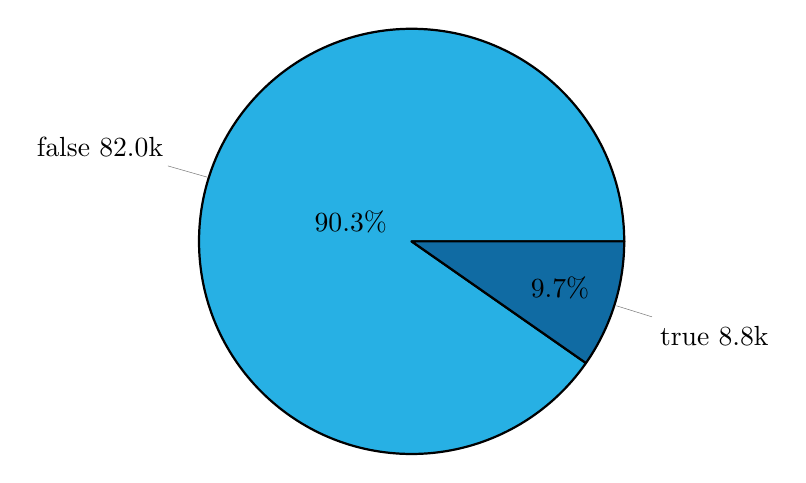
\begin{tikzpicture}[scale=0.9]
		\pie[color={myblue, mygrey}, text=pin]{90.3/false 82.0k, 9.7/true 8.8k}
	\end{tikzpicture}
\end{center}
	
	\subsubsection{Oversampling vs Undersampling}
	
	\section{Machine Learning}

	\section{Analisi esplorativa dei dati}
	
	\section{Conclusioni}
	

	
\end{document}